\RequirePackage[l2tabu, orthodox]{nag}
\documentclass[a4paper,parskip=half]{scrartcl}
\usepackage[english]{babel}
\usepackage[T1]{fontenc}
\usepackage[utf8]{inputenc}
\usepackage[pdftex]{graphicx}
\usepackage{mdwlist}
\usepackage{array}
\usepackage{multirow}
\usepackage{textcomp}
\usepackage{float}
\usepackage{xspace}
\usepackage{rotating}
\usepackage{bytefield}
\usepackage[pdftex,dvipsnames,table,xcdraw]{xcolor}  % Coloured text etc.
\usepackage[activate={true,nocompatibility},stretch=10,shrink=10,factor=1100,babel=true]{microtype}

\usepackage{tikz}
\usepackage{tikz-qtree}
\usetikzlibrary{babel,arrows,positioning,calc,fit}

\PassOptionsToPackage{hyphens}{url}\usepackage[hidelinks]{hyperref}
\usepackage[compatibility=false]{caption}
\usepackage{subcaption}

\usepackage{minted}
\usemintedstyle{autumn}
% \usemintedstyle{bw} % use for black and white
\newminted{java}{gobble=1,linenos,numberblanklines=false,frame=lines,tabsize=4}
\newminted{c}{gobble=1,linenos,numberblanklines=false,frame=lines,tabsize=4}
\newminted{xml}{frame=none,tabsize=1,fontsize=\small}
\newminted{cpp}{frame=lines,tabsize=4}

\usepackage{xpatch,letltxmacro}
\LetLtxMacro{\cminted}{\minted}
\let\endcminted\endminted
\xpretocmd{\cminted}{\RecustomVerbatimEnvironment{Verbatim}{BVerbatim}{}}{}{}

\usepackage[nameinlink]{cleveref}

\usepackage{xargs}  % Use more than one optional parameter in a new commands
%
\usepackage[colorinlistoftodos,prependcaption,textsize=tiny]{todonotes}
\newcommandx{\change}[2][1=]{\todo[linecolor=Bittersweet,backgroundcolor=Bittersweet!25,bordercolor=Bittersweet,#1]{#2}}
\newcommandx{\improvement}[2][1=]{\todo[linecolor=Orange,backgroundcolor=Orange!25,bordercolor=Orange,#1]{#2}}
\newcommandx{\unsure}[2][1=]{\todo[linecolor=Green,backgroundcolor=Green!25,bordercolor=Green,#1]{#2}}
\newcommandx{\info}[2][1=]{\todo[linecolor=blue,backgroundcolor=blue!25,bordercolor=blue,#1]{#2}}
%

\newcommand{\bitlabel}[2]{%
\bitbox[]{#1}{%
\raisebox{0pt}[4ex][0pt]{%
\turnbox{45}{\fontsize{7}{7}\selectfont#2}%
}%
}%
}

\newcommand{\colorbitbox}[4]{%
\rlap{\bitbox[]{#2}{\color{#1}\rule{\width}{\height}}}%
\bitbox[#4]{#2}{#3}}

\definecolor{mygreen}{HTML}{097054}
\definecolor{myyellow}{HTML}{FFDE00}
\definecolor{myblue}{HTML}{6599FF}
\definecolor{myorange}{HTML}{FF9900}

\newcommand{\nocontentsline}[3]{}%
\newcommand{\tocless}[2]{\bgroup\let\addcontentsline=\nocontentsline#1{#2}\egroup}%

% Abbreviations
\newcommand{\java}{{\small Java}\xspace}
\newcommand{\python}{{\small Python}\xspace}
\newcommand{\cpp}{{\small C++}\xspace}
\newcommand{\xmlmate}{\textsc{XMLmate}\xspace}
\newcommand{\evosuite}{\textsc{EvoSuite}\xspace}
\newcommand{\xml}{{\small XML}\xspace}
\newcommand{\xsd}{{\small XML Schema Definition}\xspace}
\newcommand{\xom}{{\small XOM}\xspace}
\newcommand{\pin}{{\small Pin}\xspace}
\newcommand{\pcap}{{\small pcap}\xspace}
\newcommand{\png}{{\small png}\xspace}
\newcommand{\zmq}{{\small ØMQ}\xspace}
\newcommand{\msgpack}{{\small MessagePack}\xspace}
\newcommand{\xerces}{{\small Xerces2}\xspace}


\begin{document}
\begin{titlepage}
\begin{center}
{\LARGE \bfseries Saarland University \\
Faculty of Natural Sciences and Technology I \\[0.1cm]
Department of Computer Science}\\[2.5cm]

{\Large \bfseries Master's Thesis}\\[1cm]
{\LARGE \bfseries Something something something\ldots XMLMate}\\[2cm]
{\small \bfseries submitted by}\\[0.5cm]
{\large \bfseries Nikolas Havrikov}\\[1cm]
{\small \bfseries submitted on}\\
20.03.2015\\[2.5cm]
{\bfseries Supervisor}\\[0.2cm]
Prof. Andreas Zeller\\[1cm]
{\bfseries Advisor}\\[0.2cm]
Matthias Höschele\\[1cm]
{\bfseries Reviewers}\\[0.2cm]
Prof. Andreas Zeller\\[.2cm]
Dr. Christian Rossow
\end{center}
\end{titlepage}
\newpage
\begin{center}
{\LARGE \bfseries Eidesstattliche Erklärung}\\[0.2cm]
Ich erkläre hiermit an Eides Statt, 
dass ich die vorliegende Arbeit selbstständig verfasst und keine anderen als die angegebenen Quellen 
und Hilfsmittel verwendet habe.\\[1cm]
{\LARGE \bfseries Statement in Lieu of an Oath}\\[0.2cm]
I confirm under oath that I have written this thesis on my own and that I 
have not used any other media or materials than the ones referred to in this thesis.\\[3cm]
{\LARGE \bfseries Einverständniserklärung}\\[0.2cm]
Ich bin damit einverstanden, dass meine (bestandene) Arbeit in beiden Versionen in die 
Bibliothek der Informatik aufgenommen und damit veröffentlicht wird.\\[1cm]
{\LARGE \bfseries Declaration of Consent}\\[0.2cm]
I agree to make both versions of my thesis (with a passing grade) accessible to the public 
by having them added to the library of the Computer Science Department.\\[3cm]
\end{center}
\vfill
\begin{flushleft}
\begin{tabular}{ll@{\hspace{4.2cm}}r}
    Saarbrücken, & \rule[-2pt]{2.9cm}{.4pt} & \rule[-2pt]{4.4cm}{.4pt} \\[0px]
     & (Datum / Date) & (Unterschrift / Signature) \\
\end{tabular}
\end{flushleft}
\newpage
\section*{Acknowledgements}
This thesis has benefited from the support of several people, whom I would like to thank sincerely.
I would especially like to thank
\begin{description}
	\item[] Andreas Zeller for providing this interesting and challenging research topic,
	\item[] Christian Rossow for suggesting lots of interesting ideas and giving good hints,
	\item[] Giorgi Maisuradze for active support during the implementation phase, as well as providing format
	converters and schema for the png format,
	\item[] Juan Pablo Galeotti for tirelessly trying to constrain the scope of the thesis,
 	\item[] Elias Hartz for rigorous feedback on the quality of this text document,
	\item[] and Joachim Couturier, Dennis Kamkar, and Thomas Konietzke for being inexhaustible sources
	of motivation and for keeping me sane during my working on this thesis.
\end{description}
\newpage
\section*{Abstract}
%%%Motivation - want find vulns when autotesting
When generating test inputs with the goal of revealing failures and vulnerabilities in a program, 
%%%Problem - inputs must be well-formed
the inputs must adhere to a format specific to this program, otherwise they are 
quickly discarded without getting anywhere near executing important logic code.
%%%Methodology - grammars + search-based + specific criteria
Several techniques can be used to profitably apply automated test input generation in this usage scenario -
they include leveraging format description grammars, employing search-based instance development algorithms,
and utilizing guidance criteria specifically designed for individual vulnerability classes.
%%%Results - prototype, subjects, failures
A prototypical implementation extending the search-based input generator \emph{XMLMate} with the suggested
techniques has been applied to several file formats and their corresponding libraries and has shown promise as
it detected failures, which have been confirmed as vulnerabilities.
%%%Optional - more details on subjects and their vulnerabilities
\newpage
\tableofcontents
\newpage
\section{Introduction}
Many applications receive input data as files. These files must usually adhere to a specific format in order
to be accepted by the application since it is common practice to swiftly discard inputs should they not pass a
conformity check. Examples of such checks include schema validation and checksum verification. Typically, these
checks are of no interest when testing such applications as the goal is rather testing the logic of the
application itself; however, they present an obstacle when generating inputs for
testing purposes.

Creating test inputs in sufficient quantities manually is often infeasible because of the overwhelming number
of values that need to be produced -- possibly in different combinations and successions -- which is why in
this case automatic testing is the only viable alternative. Several ideas can be explored to enable automatic
testing techniques to produce test inputs which pass conformity checks as well as improve the quality of the
resulting tests as much as possible.

The first idea is to leverage the same format definitions that are used for the checks when generating the
inputs. For an example consider an \xsd, which describes the format of a concrete \xml dialect, it contains all
the information necessary to generate instances of this dialect; another example -- the \png file format
documentation, which describes all values that are legal in \png files.

The second idea is to occasionally ignore some parts of the specification with the goal of producing inputs
that reveal vulnerabilities in the application under test. This is especially important as all such exposures
present a real threat to security or usability because tests of real usage scenarios (i.e.\ system level tests)
cannot produce false positives by definition.

The third idea is to benefit from search-based techniques when generating test inputs in order to increase
effectiveness by steering the production of inputs towards desired properties or particular testing goals like
specific classes of security vulnerabilities.

\xmlmate{}\cite{Havrikov:2014:XEX:2635868.2661666} is a tool that already implements most of these ideas to
some extent -- it is capable of generating \xml instances from an \xsd{}, and optionally additional \xml
samples, using a search-based genetic algorithm based on \evosuite{}\cite{fraser2013whole}. \xmlmate is
primarily aimed at \java applications that process \xml files, however, it is very well-suited to be extended
to work with non-\java programs, non-\xml formats, and vulnerability-oriented guidance criteria for the
search-based input generation algorithm.

The goal of this thesis is to provide \xmlmate with prototypical implementations of these extensions and
evaluate their effectiveness and efficiency on several test subjects, and thus determine the viability of the
proposed ideas for enhancing test input generation techniques in the context of automated system testing.

% TODO Add short schematic description of proposed implementations and an illustration

The remainder of this document is organized as follows: \cref{sec:relwork} gives an overview of approaches
related to the one proposed, which is described in great detail in \cref{sec:approach}, including the
technology stack used, the components the system consists of, challenges encountered during implementation and
their solutions, as well as guidance function and file format descriptions. The evaluation setup and
experimental results are presented in \cref{sec:evaluation}, whereafter \cref{sec:conclusion} provides a
conclusion statement, which is followed by an outlook on future enhancements and challenges in
\cref{sec:future}.

\section{Related Work}
\label{sec:relwork}
There is an entire class of approaches which put an emphasis on the diversity of the produced inputs and the
efficiency of their generation over guidance towards any certain criterion. These are collectively known as
\emph{fuzzers}, typically their primary goal is to find failures and vulnerabilities, and they can be
categorized as follows.
\subsection{Blackbox Fuzzers}
Blackbox fuzzers have no knowledge of the application they are testing whatsoever -- they simply generate random
inputs that can be fed into the program under test to see if it can handle the input or if it crashes.
There are many tools that can be at least partially classified as blackbox fuzzers. For \xml-based formats
there are the integrated development environments Eclipse\cite{eclipse} and Visual Studio\cite{visual} which
are both capable of generating simple instances for a given \xsd. The oXygen\cite{oxygen} tool is a
dedicated stand-alone \xml instance generator, which makes it, in contrast to the previous examples, a true
fuzzer.
 		 
The TAXI\cite{Bertolino:2007:ATD:1270230.1270257} approach presents a variation on the same principle, but
offers an improvement by making use of partition testing: the number of instances to be generated
and tested can be significantly reduced under the assumption that the ranges of values specified in the \xsd
can be divided into partitions, such that if the application under test can accept and handle one input from a
partition, it can do so with all the other values from the same partition.

Wuzhi Xu et al.\cite{1544740} have applied blackbox fuzzing on web services and extended the approach by
performing perturbations on the \xsd before generating instances in order to additionally test the resilience
of the validation mechanism.

Codenomicon Labs have developed a proprietary XML fuzzing framework\cite{codenomicon} as part of their
\textsc{cross} initiative (Codenomicon Robust Open Source Software). According to their own description their
fuzzer is capable of introducing various kinds of malformities into the generated inputs -- breaking the
encoding, repetition of tags and elements, dropping of tags and elements, recursive structures, overflows,
special characters, and many others.

\subsection{Whitebox Fuzzers}
In contrast to blackbox fuzzers, the whitebox fuzzers have some knowledge of the application under
test, which they use to get some degree of feedback on the inputs they generate. They mostly use this feedback
to refrain from generating duplicates, or inputs which induce the same behavior in the tested program, thus
avoiding useless work effort and making testing more efficient.

Named after the rabbit breed ``American Fuzzy Lop", \emph{afl-fuzz}\cite{afl} is a whitebox fuzzer
primarily aimed at testing applications that take a binary file as input. Not unlike \xmlmate, it uses a
combination of genetic algorithm and lightweight dynamic instrumentation. Its main focus is on
efficiency, which means that while it can generate inputs for simple formats like \texttt{JPEG} reasonably
well\footnote{\url{http://lcamtuf.blogspot.de/2014/11/pulling-jpegs-out-of-thin-air.html}}, it fails
to produce more sophisticated ones like \png, which is riddled with internal consistency checksums.

The SAGE\cite{godefroid-sage} tool employs dynamic symbolic analysis of x86 binary code of the program under
test to obtain information about the inputs to be generated: while the program is executing, constraints on
the input format are gathered, whereafter a constraint solver is used to generate new inputs. SAGE requires
existing files as a seed because path explosion and shortcomings of symbolic execution can make starting with
empty inputs infeasible.

\subsection{Language-Specific Fuzzers}
As the probability to generate valid inputs that penetrate deep into the application logic without considerable
format specification efforts is usually infinitesimally small, it is sometimes preferable to constrain the
range of generated inputs by means of a grammar for a specific language.

LangFuzz\cite{holler2012} is a typical blackbox fuzzer that leverages this principle and offers a possibility
to provide input fragments, which it will then attempt to make use of in the process of input generation.

In their later work \cite{Godefroid:2008:GWF:1375581.1375607} the authors of SAGE have extended the approach to
take a grammar for input generation; however, their extension does not benefit from any existing inputs for
grammar-based test generation seeding.

\subsection{Search-Based Testing}
In the category of search-based approaches, i.e.\ those that employ some form of guidance criteria to steer the
generation of test data in the desired direction, there are approaches conceptually close to \xmlmate.

\evosuite{}\cite{fraser2013whole} is a dedicated unit test generator aimed at \java programs. By
dynamically observing the execution of the application under test and aiming for maximum code coverage, it
utilizes a genetic algorithm to generate entire JUnit test suites. It provides multiple code coverage
criteria as search goals, which makes it a very versatile tool. In fact, the implementation of \xmlmate is
in part based on \evosuite.

\textsc{Exsyst}\cite{gross-issta2012} is also based on \evosuite, but it specializes in testing of \java
GUI applications by generating series of interactions that aim to explore and test as many of the program's
features as possible. The result is not a test suite, but rather a set of executable GUI interactions that
provide considerable code coverage, or even reveal failures. In contrast to pure \evosuite, this approach
performs testing on the system level by exercising the tested application via the same interface as its
intended users, this means that any failure found by \textsc{Exsyst} is a real failure and not a false
positive. \xmlmate, also being a system level tool, has this property as well.
\section{Approach}
\label{sec:approach}
The work presented in this document mainly consists of adding new features and areas of application to the
prototypical \xmlmate implementation, thus increasing its value for automatic test generation use cases. The
most significant extensions include 
\begin{description}
\item[]adding support for applications not running on the \java virtual machine by using an x86 binary code
dynamic instrumentation to be able to analyze any x86-based programs including popular libraries and rendering
engines.
\item[]extending support for pluggable fitness functions to allow for narrow-scope application contexts such as
scanning the targeted program for specific classes of defects or vulnerabilities.
\item[]adding more output formats to both demonstrate the versatility of the original approach as well as
increase the set of applications compatible to be tested with \xmlmate.
\end{description}

Yet another goal of this work is performing a case study on the libpng image file rendering library to evaluate
the efficacy and efficiency of the presented extensions.
%### 
\subsection{Technology Stack}
%### 
\label{sec:tech}
Over the time of its development \xmlmate has amassed quite a technology stack, 
which has grown to include not only a number of \xml processing libraries, but also communication, instrumentation, and serialization frameworks. 
In the following sections I would like to give a brief overview of the technologies used.
%###  
\tocless\subsubsection{Xom}
%### 
\xom{}\cite{xom} is a \java library for handling \xml documents at the core of \xmlmate. 
It offers in-memory representation of \xml tree structures as well as support for Namespaces in \xml, {\small XPath 1.0}, {\small XSLT 1.0}, 
{\small XInclude}, {\small xml:id}, {\small xml:base}, Canonical \xml, and Exclusive Canonical \xml.
I decided for it in favor of {\small SAX}, {\small StAX}, {\small DOM4j} and {\small jDOM} because of its simplicity and efficiency.
It is also the only \xml API that ensures correctness very strictly - \xom only allows to create namespace well-formed XML documents, 
which coincides with one of the underlying principles of \xmlmate{} - generating valid and well-formed data.
Furthermore, \xom is open to extension, which allows for easy enhancements and adaptations to make it suitable 
for building the basis of genetic representations of \xml trees (further described in \cref{sec:repr}).

If needed, you can skip ahead and take a look at \cref{lst:xmlexample} in \cref{sec:formats:pcap}
to gain a better understanding of the kinds of file formats \xom offers support for.
%### 
\tocless\subsubsection{Xerces2}
%### 
\xerces{}\cite{xerces} is a \java library for parsing, validating and manipulating XML documents, which most
importantly to \xmlmate, has support for W3C XML Schema 1.1 (Working Drafts, December 2009).
At the heart of \xmlmate lies a representation of an \xsd, which is used as a blueprint for generating new
\xml instances and modifying existing ones. This representation is implemented with \xerces, as at the time of
conception it was really the only available \xsd implementation for \java. \xerces mainly provides access to
the definitions of a schema as well as a mechanism for validating \xml instances. Unfortunately, it only
exposes its functionality via \java interfaces, which makes enhancements and adaptations rather hard, but not
impossible, as you will see in \cref{sec:repr}.

For an impression of what an \xsd looks like in its textual form, feel free to consider \cref{lst:xsdexample},
as well as \cref{lst:repr} for its role in the genetic representation of an \xml chromosome.
%### 
\tocless\subsubsection{PIN}
%### 
{\small Intel} \pin\cite{Luk05pin:building} is a dynamic binary instrumentation framework for the IA-32 and x86-64 instruction-set architectures 
that enables the creation of program analysis tools, which perform the instrumentation at run time on  
compiled binary files. Thus, it requires no recompiling of source code and can support instrumenting programs that dynamically generate code.
\pin allows a tool to insert arbitrary code (written in {\small C} or \cpp) in arbitrary places in the executable, for which it 
provides an API that abstracts away the underlying instruction-set idiosyncrasies and allows context information 
such as register contents to be passed to the injected code as parameters. It also automatically saves and restores 
the registers that are overwritten by the injected code so the application continues to work.

Generally, the instrumentation with \pin consists of two components: a mechanism that decides where and what code to insert, 
and the code to be executed at insertion points. These two components, called \emph{instrumentation} and \emph{analysis} 
code are hosted in a single executable called a \emph{pintool}, which functions like a plugin to the \pin framework.
A pintool can register callbacks on different levels of granularity, varying from single instructions over procedures
to entire binary images, in order to receive context-dependent information and access to values of particular interest.

\pin provides two modes of execution: just-in-time (jit) and probe. The latter is designed for replacing
entire individual routines and offers a very small API, but relatively good performance. The former provides
a rich API and access to granularity levels much more precise than routine level, but the instrumented process
suffers a significant performance penalty. For the purpose of using \pin as part of specific fitness functions
a high level of detail is necessary, which is why jit mode is used. To somewhat compensate for the performance
loss, a system has been put in place, which allows to parallelize the execution of processes instrumented with
\pin. \Cref{sec:par} gives more details about these parallelization efforts.

At one point, the GNU test coverage tool \texttt{gcov}\cite{gcov} was considered as an alternative to using
\pin, yet the decision finally rested with \pin because gcov is inferior in many points: it is only
compatible with code compiled with \texttt{GCC} using debug flags and with optimizations turned off, and it
lacks the rich API that \pin offers as it is merely capable of indicating lines of code that were executed, and
thus is severely lacking in features.

There was also a consideration to use \texttt{Valgrind}\cite{Nethercote03valgrind:a} instead of \pin, but \pin
won this case as well, though mostly due to its more easily accessible and example-rich documentation. 
%### 
\tocless\subsubsection{ZeroMQ}
%###
\label{sec:zmq}
{\small ZeroMQ}\cite{zmq} (or \zmq as it as actually called) is an extremely efficient messaging library, 
which is very well suited for use in concurrent or distributed applications. \zmq regards messages as 
completely transparent blobs of data which are to be transported across predefined communication channels 
between sockets. Rather than unnecessarily defining its own transfer protocol, \zmq works on top of already exiting 
ones like \texttt{inproc}, \texttt{IPC}, \texttt{TCP}, \texttt{TIPC} and multicast such as \texttt{pgm} or \texttt{epgm}.
Out of the box \zmq provides its users with several communication patterns that can be either used directly or combined 
into more complex patterns, which remain easy to manage and use. Some basic patterns are \texttt{Request/Response}, 
\texttt{Publish/Subscribe}, or \texttt{Push/Pull} among others.
There are implementations of \zmq in many programming languages, of which the ones for \java, \python, {\small C}, 
and \cpp are actually used in \xmlmate. 

It is very easy to get started with \zmq in all programming languages - the basic concept is the
same everywhere: the program that uses \zmq must first set up a so called \emph{context}, which then becomes
host to \emph{sockets}, which, in turn, are either bound or connected to \emph{endpoints} of some transport
channel. A socket can have arbitrarily many ingoing and outgoing connections and \zmq automatically reconnects
it to any peers in case the underlying connection gets interrupted. Furthermore, a socket can be either bound
or connected to its endpoint with \emph{binding} being preferred when the component behind the socket is a
static component of the overall system; only one socket can be bound per endpoint. Conversely, a socket is
\emph{connected} when the component behind it is more dynamic in nature and may leave and rejoin the system
arbitrarily, or when the number of instances of this component is not known a priori. Sockets joined at
different ends of a connection must use different methods, in practice, this means that on one end of the line
there is a single bound socket, and on the other there is a variable number of connected sockets, which may
come and go during runtime.

There are different types of sockets: \texttt{PUB}, \texttt{SUB}, \texttt{REQ}, \texttt{REP}, \texttt{PUSH}, 
\texttt{PULL}, as well as some other, more exotic types. The different types of sockets can be plugged together
like their names suggest, for example \xmlmate combines a multitude of \texttt{PUSH} and \texttt{PULL} sockets
to create a processing pipeline for its \xml files and their fitness scores.

Beside \zmq there are other messaging solutions, some of which were considered for use in \xmlmate. One such
library is {\small RabbitMQ}\cite{rabbitmq} - it implements the AMQP protocol and as such requires a central
message broker. This means an additional process in need of customization and deployment would be needed, and
writing client side code is also somewhat more difficult; this is why {\small RabbitMQ} was decided against.

Then there is {\small nanomsg}\cite{nanomsg}, which was written by one of the authors of \zmq. 
It is similarly brokerless, more lightweight and efficient than \zmq, and has an even easier to use API, which
for example does not burden its users with the concept of a context; however, it is still in beta and lacks
the gigantic community support like that of \zmq, which ultimately lead me to not choosing it either.
%### 
\tocless\subsubsection{MessagePack}
%### 
\label{sec:msgpack}
Because a messaging library only solves the problem of getting \emph{arbitrary data} between peers, it 
alone does not suffice for creating a fully fledged communication protocol - this is where
serialization/deserialization libraries usually come in. \msgpack{}\cite{msgpack} is one such serialization
format that is highly efficient as it uses binary representation of data. It is implemented as a library in at
least 20 programming languages. Once again, \xmlmate uses the ones for \java, \python, {\small C}, and \cpp.
While \msgpack is very efficient in what it does, it has some disadvantages such as 
\begin{itemize}
  \item Integer values are limited to be in $[-2^{63}, 2^{64}-1]$.
  \item The maximum length of an array or string is limited to $2^{32}-1$.
  \item It is the user's responsibility to ensure correct endianness across all endpoints.
\end{itemize}

There is another relatively young binary serialization format
{\small CBOR}\footnote{\url{http://tools.ietf.org/html/rfc7049}} that does not have many of {\small
MessagePack's} disadvantages, while being comparatively as efficient.
There are implementations in {\small C}, \python and \java; however, at the time of {\small XMLMate's}
conception I did not know of their existence. 
% C (https://github.com/upwhere/ccbor), 
% Python (https://code.google.com/p/cbor/) 
% and Java (https://github.com/c-rack/cbor-java)
After some additional research more serialization/deserialization formats and libraries were found, like
{\small Cap'n Proto}\footnote{\url{https://capnproto.org/}},
{\small Simple Binary Encoding}\footnote{\url{https://real-logic.github.io/simple-binary-encoding/}}, and
{\small FlatBuffers}\footnote{\url{https://google.github.io/flatbuffers/}} with some more promising than
others. Finding a more suitable replacement for \msgpack might be a subject of some future enhancement.
%### 
\tocless\subsubsection{GNU Trove}
%### 
\label{sec:trove}
The GNU Trove \java library provides performant and memory efficient alternative implementations of the
standard \java collections API, and, in addition, offers collections supporting primitive types. 

A disadvantage of \java's standard collections, which can often quickly become a performance bottleneck in
applications that handle lots of primitive values, is their lack of direct support for those. In
order to store primitive values in the standard collections, it is necessary to envelop each and every single
value in its own wrapper object - a process known as \emph{boxing}, which incurs costs both in memory use and
computing time. This practice is so common that since version $1.5$ \java offers autoboxing functionality,
whereby programmers can put primitive values where their wrapper counterparts are expected and vice versa, and
the \java compiler would perform the necessary boxing and unboxing automatically, thus hiding the additional
cost from inexperienced programmers. In most cases, these additional costs can be calmly neglected, but
sometimes they cannot. In order to exclude the possibility of this becoming a problem and suddenly sneaking
up, the decision was made to go with Trove collections from the beginning. These collections have since found
their special use with the many details of the various evaluation result types, e.g. storing big amounts of
memory addresses.
%### 
\subsection{System Components}
%### 
\label{sec:components}
Extending \xmlmate to support binary subjects has greatly benefited from frameworks described in
\cref{sec:tech} as they help solve the majority of the arising subtasks rather elegantly. The following
paragraphs describe the components involved in the new extended \xmlmate work process.
%###  
\paragraph{XMLMate Core} ~\\
%### 
  The \java application \xmlmate performs its genetic operations on a population of chromosomes; this 
  results in a set of \xml files, whose fitness needs to be determined according to the currently employed
  fitness function. The paths to these files are then sent out via a \zmq socket either directly to the
  \emph{test drivers}, in case the program being tested supports reading inputs in \xml format, or alternatively 
  to an arbitrary number of \emph{converters}, that, as the name suggests, convert the \xml files into a format 
  suitable for the system under test. This distinction is completely transparent to \xmlmate and thus allows for 
  adding an arbitrary number of transformation steps between itself and the test drivers.
  %### 
  \paragraph{Load Balancer} ~\\
  %### 
  A load balancer is responsible for managing a set of homogeneous worker nodes like converters or test
  drivers by distributing the arriving workloads fairly among them. The fair queueing provides a significant
  performance upgrade from the previously employed round robin method. Not all workloads require equal
  processing time, and because it is indeterminable a priori, the round robin workload distribution strategy
  has often caused faster work items to get ``stuck'' in queue behind slower ones, while there were idle
  workers available. The new load balancing mechanism allows to track the worker's availability and assign
  newly arriving workloads to idle workers in the least recently used order. To provide an analogy, the load
  balancer's queueing strategy has been upgraded from a supermarket to a post office. 
  
  A load balancer provides a facade for the workers it manages, so that other system components only ever
  directly interact with the balancer, but never with the workers themselves, as they are sometimes unreliable
  and can fail at any moment. The most common system setup consists of two load balancers -- one for the format
  converters and one for test drivers, so even though it says above that \xmlmate sends its work packets to
  converters or test drivers, in actuality it communicates with their respective load balancers. 
  %### 
  \paragraph{Format Converter} ~\\
  %### 
  A format converter (most of which are currently implemented in \python) receives a conversion task from
  its load balancer through a \zmq socket, which it completes by converting the file found at the location
  specified in the task message. It then responds with another message containing the location of the converted
  file. There can be an unlimited number of converters active at the same time processing multiple
  conversion requests in parallel. 
  
  The design decision to enable the converters to drop in and out at
  runtime has two very useful properties: firstly, it allows to circumvent the parallelism limitation
  imposed by Python's GIL (global interpreter lock) by being able to run multiple interpreter
  instances in parallel without them interfering; and, secondly, it makes it possible to apply meta-heuristics
  to the process by varying the number of converters dynamically depending on the load, which makes for an
  interesting future work item.
  %### 
  \paragraph{Test Driver} ~\\
  %### 
  A test driver receives a message from its balancer, which, in turn, receives it either directly from
  \xmlmate in case of an \xml based file format, or otherwise from the previous balancer (usually a
  converter's balancer), unpacks the file path, and feeds it to the system under test, which is being monitored
  by a \emph{pintool} that implements the ``client side" of the aforementioned currently employed fitness
  function. The test driver's responsibilities also include signaling the beginning and end of the execution of
  the program under test to the pintool by calling special marker methods \texttt{PIN\_SCORE\_START}
  and \texttt{PIN\_SCORE\_END}, which the pintool replaces with its own internal fitness data related
  processing methods. The driver is implemented in C and, as is the case with converters, there can
  be arbitrarily many active at the same time.
  %### 
  \paragraph{Pintool} ~\\
  %### 
  As previously mentioned, the pintool monitors the execution of the program under test and records
  data relevant to the computation of the fitness score according to the fitness function it is part of.
  E.g.\ for a fitness function that counts the number of basic blocks executed in the program, the pintool 
  would keep a set of basic blocks that it has observed being executed. The pintool replaces the call to 
  \texttt{PIN\_SCORE\_START} in the driver with a method that resets its fitness related data stores. In the 
  above example this would clear the set of executed basic blocks. The pintool also replaces the call to
  \texttt{PIN\_SCORE\_END} with a method that sends the stored data back to the balancer. 
  The pintools are implemented in \cpp and there is always exactly one pintool per test driver.
  Because each pintool runs in the same process as its test driver, it is possible to share the same \zmq
  socket between driver and pintool to communicate with the load balancer, which makes it relatively
  easy to implement the next system component.
  %### 
  \paragraph{Lifeguard} ~\\
  %### 
  A lifeguard protects the joint process of test driver, system under test and pintool from fatal application
  crashes. Whenever \xmlmate produces an input file which crashes the program under test, the entire process
  dies off without a possibility to report this valuable finding. To prevent this, a lifeguard launches a
  driver process and gives it an \emph{identity} (which is a \zmq concept -- the load balancer distinguishes
  the workers by their identities). As soon as control returns to the lifeguard, which means that the launched
  process has died, it assumes the identity of the recently deceased and reports the fact of death to the load balancer, which will transparently forward this to \xmlmate in order for the corresponding input to be
  stored. Afterwards, the lifeguard casts off the identity and relaunches the driver with it once again.
  Each test driver is being guarded by its own personal lifeguard implemented in \python.
  %### 
  \paragraph{Fitness Function} ~\\
  %### 
  The fitness function in \xmlmate receives the message from the pintool and interprets it according to 
  its specification. E.g.\ again, if the fitness function is supposed to count the number of executed basic
  blocks, it would expect to receive a set of basic block addresses. Finally, the  fitness function assigns the
  computed fitness score to the genetic representation of the \xml file sent out in step 1, unless the message
  says that the corresponding input has caused a test driver to die, in which case the genetic representation
  will receive the worst fitness score to be removed from the population in order not to continuously keep
  crashing the test drivers, and the input file itself will be kept permanently.

%### 
\paragraph{Overview} ~\\
%### 
\Cref{fig:components} provides a schematic overview of the aforementioned components and which other components 
they interact with inside the system. The visualization also shows that the system scales out to \texttt{n}
format converters and \texttt{m} \emph{workers} --
a collective noun summarizing a test driver, its pintool, the program under test, and their lifeguard
instance.

\begin{figure}[htb]
\centering
  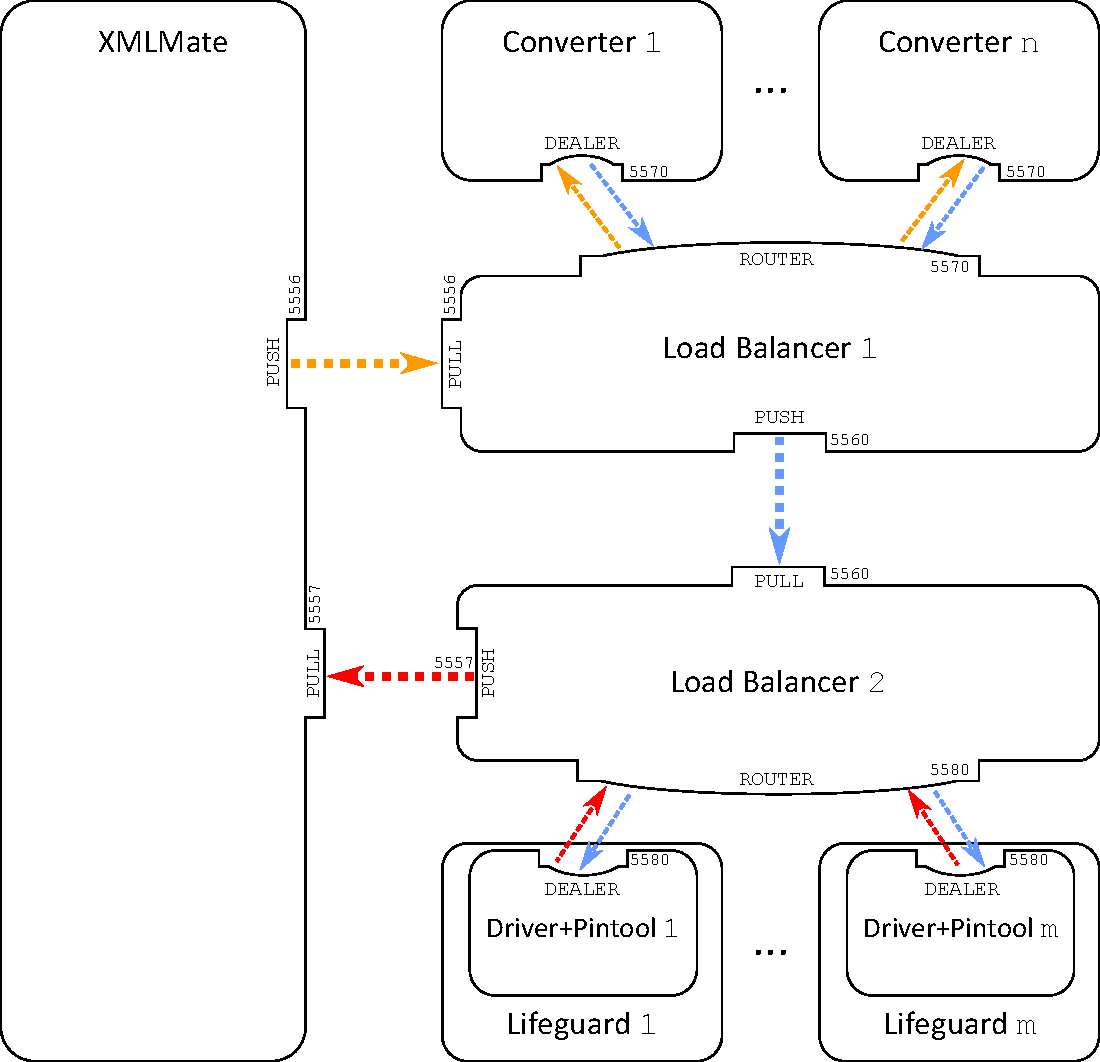
\includegraphics[width=\columnwidth]{system.pdf} 
  \caption{The Components of \xmlmate. 
  The arrows indicate the flow of data between the system components. Orange arrows denote the work items
  in \xml format sent out by \xmlmate itself, the blue arrows show the flow of converted files, and the red
  arrows signify the way the fitness information takes.
}
  \label{fig:components}
\end{figure}

%### 
\paragraph{Development Mockups} ~\\
%### 
When developing such a diverse ecosystem it is important to be able to inspect and test each component
individually, so as not to lose track of any important details, and to be able to isolate faults efficiently
without having to keep the entire system in the focus of attention. 
This is best accomplished by constructing
very lightweight mockup versions of the most important system components, so that the entire system does not
have to be launched when concentrating on a single component. Instead, only the single real component under
investigation has to be started, while the rest of the system is being simulated by the ``bare bones''
component mockups.

Examples for such mockup components that were used during development include two test driver mockups -- one
written in \java and one in C, which were used to test basic \zmq connectivity and
cross-language \msgpack serialization/deserialization respectively. Several mockups for the system under test
were used to test the \java parts of \xmlmate's fitness functions by simply sending random data in the
required \msgpack format without requiring any binary instrumentation. There is also a mock version of
\xmlmate itself, which sends out work items that consist of hardcoded file paths, alleviating the need to
constantly generate new input files, as well as providing deterministic inputs as a means to test the
consistency of values reported by the pintool components of fitness functions. Having this mockup send out
predefined work items also allows to skip the format conversion phase, which further lightens the complexity
of the system.

In most cases, when implementing new components of a system from scratch, I found it to be very advisable to
start with their mockup version, as the effort is usually worthwhile since any mistakes can be caught
cheaply and early on and most of the code is directly transferable to the finished component.
\FloatBarrier
%###
\subsection{Challenges}
%###
Getting away from pure \java and adding support for application binaries as test subjects 
to \xmlmate by transforming it from 
a single \java application into a set of loosely coupled, yet interdependent and distinct 
processes written in different programming languages presented a number of challenges from 
such fields like software engineering and system architecture design. 
In the following sections I would like to shed some light onto 
the most noteworthy of them.
%###
\subsubsection{Chromosome Representation}
%###
\label{sec:repr}
\xmlmate is implemented on top of the genetic algorithm framework that is part of 
\evosuite\cite{6004309} and as such must adhere to its specifications and structures 
of genetic representations. 
Because \evosuite as a whole is aimed at generating {\small JUnit} tests for \java applications, 
the entities that comprise the population  (i.e. the \emph{chromosomes} or \emph{individuals}) 
are called \emph{test suites}. The test suites are what evolves from generation to generation.
In turn, the test suites consist of \emph{tests}. Similarly, \xmlmate has adopted the concepts of 
test suite and test they correspond to a set of \xml trees and a single \xml tree, respectively. 
They are sometimes referred to as \emph{test suite chromosomes} and \emph{test chromosomes}, resp.


In \xmlmate all \xml trees are governed by a single \xsd that is given as a parameter at program start.
In order to implement the genetic operation \emph{mutation} for test chromosomes more or less 
efficiently each node in a test's \xml tree should have a reference to its corresponding definition 
in the schema. This is accomplished by extending some of the \java classes provided by \xom to include the 
references in question as well as methods that maintain their relevance and correctness. This alone, 
however, is not sufficient for implementing an effective \emph{crossover} of two \xml trees.

To quickly find sites suitable for crossover in two test chromosomes an additional mapping is needed: 
one that maps definitions in the global schema to nodes that are actually present in the \xml tree, so 
as to be able to find compatible intersections.
Since I am using \xerces for storing and accessing the schema information, and it is only exposed via 
a \java interface, it was not possible to add this mapping to local copies of the schema  
enhanced with the needed references to test chromosomes. However, what could be added were local 
maps referencing the global definition instances as keys and local nodes as values. A disadvantage 
is that additional methods had to be added to ensure the relevance of these mappings, 
as the node composition of an \xml tree is constantly changing. 
One benefit of this approach is the reduced memory consumption as the schema
definition must only be stored once globally, and the local mappings are nothing but sets of references 
internally and thus very lightweight.
\improvement[inline]{Add a picture of chromosome representation}
%### 
\subsubsection{Communication Protocol}
%###
Since \xmlmate now comprises several processes, a communication protocol must be put in place to 
interconnect the individual components. The communication channels themselves are built on top of
the \zmq messaging library with \msgpack as the serialization/deserialization engine. The current
implementation uses tcp loopback\footnote{TCP loopback is used because the pure \java implementation 
of \zmq does not support \texttt{ipc} on the Windows platform, which I do most of the development on.
Using a JNI based Java wrapper as a drop-in replacement would alleviate this problem, 
but it is not considered to be worth the effort.} 
as a carrier for the messages; however, it is entirely possible
to change this to inter-process communication just by changing a configuration option, should it 
become necessary. As yet, it is very far from being a bottleneck.


After each evolution step a test suite usually contains several tests that changed due to mutation and
crossover. When the fitness of the suite is requested to be computed next time by the genetic algorithm, 
only the tests that changed should be evaluated. For each of those a file is written and a packet is 
formed consisting of a number identifying the test inside the test suite and the path to its corresponding 
file. This packet is serialized into a byte string with \msgpack and then sent as a \zmq message via a 
\texttt{PUSH} socket on a well known port (e.g. the default is 5556). After all messages have been sent,
a response is awaited for each of those sent out tasks. Responses are collected as \zmq messages coming 
in via a \texttt{PULL} socket on another well known port (default 5557) and deserialized with \msgpack 
into the identifying number and whatever data format is expected by the current fitness function. 
(E.g. a fitness function that counts the number of executed basic blocks expects an array of addresses.)
As far as the \java part of \xmlmate is concerned this is all it ever sees of the entire process, and so it 
must rely on the pintool monitoring the application under test to collect and send back fitness results.


A format converter receives a \zmq message via \texttt{PULL} on port 5556, unpacks it with \msgpack, 
stores the identifying number, converts the file, packs the stored number followed by the path to 
the converted file with \msgpack into another \zmq message and sends it out via \texttt{PUSH} on port 5560.


The broker is very simple: it pulls in messages on port 5560 and pushes them out again unaltered on port 5570.


A test driver listens on port 5570 (or 5556 if there are no converters) for incoming \zmq messages and unpacks
them with \msgpack into the identifying number and a path. It then calls \texttt{PIN\_SCORE\_START()} to 
signal the start of the execution of the system under test to the monitoring pintool, whereafter it passes the 
received file path to the sut for execution. When the sut finishes and control returns to the test driver, 
it calls \texttt{PIN\_SCORE\_END(number)} with the number stored from the message earlier.


When a test driver calls \texttt{PIN\_SCORE\_START()}, the call gets replaced with a call to a method in the 
pintool that clears its internal information buffers, thereby resetting all currently gathered fitness related 
information. When the test driver then calls \texttt{PIN\_SCORE\_END(number)}, this call gets replaced with 
one that packs and sends out a message containing the identifying number and any fitness information via \zmq 
\texttt{PUSH} on port 5557.

Please note that all ports mentioned above are customizable and even the message carrier can be changed from tcp 
to any other protocol supported by \zmq, of which there are plenty.
\improvement{Mention \zmq binding and connecting and static and dynamic system components}
\unsure{mention starting synchronization}

\change[inline]{make pretty communication graph}
%###
\subsubsection{Format Converters}
%###
One of the main tasks of this work is to show that \xmlmate is versatile enough to not be limited to 
only \xml and \xml-derived formats. In order to facilitate this versatility the concept of a format 
converter has been introduced. The main goal of a converter for a specific format is to convert an 
\xml file corresponding to a schema specification into another format as specified by the purpose 
of this converter. For an example consider a converter from \xml to the packet capture format \pcap. 
This converter expects \xml files in the format corresponding to the \pcap{} \xsd and produces a 
valid \pcap file. \info{make a section reference}


\xmlmate also has support for starting out its evolution process from a given set of inputs. If the   
inputs are not available in the \xml format, they must first be converted so as to be genetically 
representable. For this use case there are reverse converters, which convert files into their 
\xml equivalent, again, according to the corresponding \xsd. For the above example a reverse converter 
could transform any valid \pcap file into its \xml representation governed by the \pcap{} \xsd.
%###
\subsubsection{Parallelization}
%###
After running the first tests on the initial \xmlmate design, which did not include any parallelization, 
it quickly became clear that both format conversion and running the program under test with \pin 
are two performance bottlenecks significantly slowing down the entire process. Considering that the 
tests were run on a multi-core machine, and only one CPU was ever doing any work, the decision was 
made to make both the conversion and evaluation steps parallel by allowing arbitrarily many 
converter and test driver instances (along with their corresponding pintools) to participate in the process. 
This was somewhat easily accomplished due to the very well thought out design of the messaging library \zmq, 
as there were only minor issues to consider - like adding the static broker component to 
manage the dynamic number of converters and test drivers.

However, after adding the aforementioned parallelization, a new bottleneck presented itself - this time 
somewhere inside the \java part of \xmlmate. Using a \java profiling tool I was able to trace the cause 
to the mutation and crossover routines, which seems logical in retrospect because both manipulate the 
in-memory representations of \xml tree structures. That alone, however, is not sufficient to cause a 
major bottleneck. \evosuite's genetic algorithm always makes backups of entire test suites as well as 
single tests before applying any genetic operation to them in order to be able to recover from an 
unfavorable outcome (e.g. decreased fitness) and roll back all changes. So each time an in-memory \xml 
tree was going to be mutated, it was deeply copied, each time two \xml trees were going to be crossed 
over, they were both deeply copied, each time an entire test suite was going to be mutated, it was 
deeply copied - each of its tests one after another, and each time two test suites were about to 
undergo crossover, both of them were deeply copied. That was what caused this particular bottleneck. 
To remedy this situation I applied the following two improvements:

The first one was adding three distinct task executors dividing the responsibilities of deeply copying, mutating and 
crossing over \xml trees. This way all three classes of tasks were enabled to run simultaneously 
no longer needing to queue up linearly one strictly after another. The mutation task executor is 
responsible for taking a single individual \xml tree, copying it and mutating the copy; the 
crossover task executor takes two \xml trees, delegates their copying to the copying task executor 
for a speed up, and then performs the actual crossover on the returned copies.

The second improvement was making the process of copying the test suites shallow instead of deep. 
This is a safe change since the individual tests are still copied before any changes are applied 
to them - the result is a kind of \emph{copy-on-maybe-write} policy as only those tests are copied 
that are going to experience potential change.

After that there were still other bottlenecks - some more surprising than others. For example 
it was rather sudden to see calls to the \texttt{Random} class being listed among the most time consuming 
by the profiler. In \java 7 the \texttt{Random} class is thread-safe, which has lead to a lot of 
contention when multiple threads suddenly started asking the singleton instance of \evosuite's randomness 
provider for random values for mutation and crossover. The fix was rather easy: \java 7 also provides 
a \texttt{ThreadLocalRandom} class intended for exactly this kind of situation; this easy fix came 
at a price, however - it is no longer possible to provide a single seed value to the whole generation 
process.

Another minor performance optimization included adding a polymorphic method for selecting a random 
element from a given \texttt{Set}. The previously available methods treated a \texttt{Set} like a 
\java \texttt{Collection} and performed the selection by first copying the entire set into a 
\texttt{RandomAccess}-able \texttt{List}. This is clearly wasteful of resources in case the set in question is large.
In this case it actually faster to generate a random number between zero and the number of elements in 
the set and then actuate the set's iterator that number of times finally claiming the element acquired 
last as the required random choice.

One further possible major optimization could be to allow partial fitness score evaluation while a suite 
mutation is still in progress. When an \xml file has left the mutation or crossover executor it could be 
immediately sent out to worker processes for fitness evaluation. Preliminary tests showed promising 
results; however, this optimization is very intrusive of \evosuite's concept of a single threaded 
genetic algorithm possibly leading to grave incompatibilities with other mechanisms deep within other parts 
of \evosuite, therefore it was deemed as a neat future work item, which should probably be combined with a 
proper restructuring of the genetic framework. \unsure{maybe mention parallel processing of test suites}
%###
\subsubsection{Local Search}
%###
As previously mentioned, one of the core principles of \xmlmate was to always create schema-valid inputs; 
however, this no longer complies with current requirements in the use case of security testing as the 
inputs that most often cause the targeted program to fail usually deviate from the specification in 
one way or another. The case where the syntactic validity of the \xml representation is violated is 
both unfavorable to format conversion and out of scope of this work.

Fortunately, it is possible to use another artifact of \evosuite's design to provide deviations from the 
specification in values (as opposed to structure): the local search. 
The local search is a mechanism which allows to perform small mutations in limited contexts in between 
the regular genetic operations to find individuals that are ``closely related'' to existing ones
yet have better fitness. One implementation of this is interval bounded numeric offset mutation whereby
several numeric values in the individual are changed by an offset chosen at random from a predefined 
interval. E.g. integer values are changed by random values from $[-10,10]$ and floating point numbers 
are offset by values from $[-0.5,0.5]$.
Performing such changes sometimes leads to the values leaving their value spaces specified in the schema, 
which allows to accommodate for the new use case of security testing.

Quite ironically, \evosuite's genetic algorithm framework for some reason does not create a backup 
copy of individuals before initiating local search, which manifested itself in abruptly diminishing 
fitness values; this was, of course, fixed by issuing a backup copy inside the local search procedure, 
additionally taking full advantage of the newly implemented parallelized deep copying mechanism.
\unsure{mention incompatibility with sec:fit:schema, and make it another small and nifty future work item}
%### 
\subsection{Formats and Subjects}
%###
\xmlmate now supports producing inputs in almost any format, provided there is an \xsd and a converter
available. Let me describe some formats that were experimented with along with their schemas, converters, and
subject programs in the next sections.
%### 
\subsubsection{XML}
%###
Before I proceed with describing other exciting formats, I want to emphasize that by being extended to an all
new multi-component distributed system \xmlmate has by no means lost its ability to interact with subject
programs that actually process inputs in the \xml format. As a matter of fact, \xml as such is not exactly a
full-fledged format in and of itself, it is rather a meta format, which many other formats are subsumed by. One
such example is the ubiquitous \texttt{html} format, which, coincidentally, I have chosen as the basis format
for testing \texttt{libxml} - a library for processing generic \xml documents written in \texttt{C}, which is
\unsure{add examples, e.g. python's lxml}
widely used as the foundation of an entire multitude of parser implementations. 
\texttt{html} has a very complex specification, which exhibits almost all of \xml's feature set.
%### 
\subsubsection{PNG}
%###
 
%### 
\subsubsection{Pcap}
%###
 
%### 
% \subsubsection{Flac}
%###
 
%### 
\subsection{Fitness Functions}
%### 
One requirement of this work was to provide \xmlmate with the concept of pluggable fitness functions and 
give several examples that demonstrate the versatility of the approach. Luckily, \evosuite already provides 
a \texttt{FitnessFunction<T extends Chromosome>} generic interface, which can be made use of on multiple 
levels of abstraction. To provide the pluggability on the level of  entire test suites there are implementers of
\texttt{FitnessFunction<XMLTestSuiteChromosome>} and on the level of single test inputs ones of 
\texttt{FitnessFunction<XMLTestChromosome>}. 
Secondary evolution objectives have a very similar type topography; secondary objectives are sometimes useful 
as ``tie breakers'' when a decision between two chromosomes has to be made when both have equal fitness values,
but possess subtle differences that e.g. might lead to slightly more or less favorable crossover behavior in 
the future. The next sections describe some of the new fitness function implementations available with the 
extended and improved \xmlmate.
%### 
\subsubsection{Schema Coverage Fitness Function}
%###
\label{sec:fit:schema}
The very first extension from pure \java branch coverage and exception oriented fitness functions employed 
previously in \xmlmate is the \texttt{Schema Coverage} fitness function. Its goal is to maximize the number 
of schema rules used in the generated inputs. The reasoning behind this is that inputs which exhibit most of 
the features described in the specification should also trigger more functionality in the program under test. 
More concretely the schema coverage fitness value is computed as the average of the folowing three values:
\begin{description}
  \item[element coverage] describes how many element declarations were instantiated in the generated inputs, 
  including substitution group members. A substitution group consists of jointly declared elements, which 
  can take each other's place in the \xml. Additionally, the element coverage can reflect how many branches 
  of choice particles as well as how many of the optional elements are present in the produced files.
  \item[attribute coverage] is, similarly, a measure of how many attribute declarations were utilized, so its 
  value depends on both the optionality of the declarations and the number of generated elements (or more 
  precisely the number of elements carrying the corresponding attribute declarations).
  \item[transition coverage] probably sounds a little out of place, so let me first explain how the concrete 
  values for elements and attributes are generated. One of the most implementation-wise challenging features 
  of the \xsd{} {\small Language} is the \texttt{pattern} facet that describes valid values of an element or 
  attribute by means of a regular expression (that has a different grammar than that of \java, \python or 
  {\small Perl} regular expression languages, which, as an aside, presented another whole technical challenge). 
  In order to be able to provide values conforming to those regular expressions an automaton based representation 
  has been put in place for the types of the elements and attributes by using the automaton
  library\cite{automaton} for \java.
  In fact, it worked so well, that there was longer any need in representing any type in a way other than by
  means of a deterministic finite automaton. This means that all types, including \texttt{string},
  \texttt{int}, \texttt{short}, \texttt{hexBinary}, have a corresponding automaton, which is cached in memory
  for performance reasons. Furthermore, with this representation it is very easy to apply additional facets
  like restrictions on length or number of fractional digits just by performing automaton based operations
  like union and intersection.
  Coming back to the topic of schema coverage, the transitions in these automata are the subject of its 
  transition coverage component which describes how many of the transitions of all the automata are being 
  used in the generated \xml files. This measure is indicative of the overall proportion of covered value space 
  over all type definitions regarded together.
\end{description}

If the element, attribute and transition coverages are designated as $c_e$, $c_a$, and $c_t$ respectively and
are numbers between zero and one, the overall schema coverage fitness value can be computed as $1 -
\frac{c_e+c_a+c_t}{3}$, which makes this a \emph{minimization} fitness function, meaning that the genetic
algorithm of \evosuite will try to get the value as close to zero as possible, which is its default behavior.

Contrary to the initial expectations, \improvement{mention in the Evaluation section} the results do not 
necessarily show a strong correlation between high schema coverage and some kinds of code coverage like 
branch or basic block coverage. This can be explained by the fact that it is not the abundance of different 
input values, but rather some specific values themselves, that are responsible for penetrating deeper into a 
program's logic and thus increasing the code coverage.

However, the schema coverage is a good evolution guide for the purpose of creating a diverse starting population
which can then be further evolved with different purposes - be it code coverage of particular program regions, or
other kinds of fitness criteria like closeness to integer overflows and the like.

Furthermore, there is no need in powering up any of the infrastructure involved with usual ways of measuring 
fitness - no system under test, no brokers or converters are needed to compute the schema coverage fitness. 
There is also no need for \texttt{IO} operations, as all \xml tree evaluations are processed in-memory.

%### 
\subsubsection{Basic Block Coverage Fitness Function}
%###
A more or less direct transfer of \evosuite's \texttt{Instruction Count} fitness function is the 
\texttt{Basic Block Coverage} fitness function, which aims to maximize the number of basic blocks 
executed in the program under test. This fitness function makes heavy use of the {\small Intel} \pin
instrumentation framework - in particular its definition of a basic block: a single entrance, 
single exit sequence of instructions in the program under test. However, because \pin is discovering the 
program dynamically as it is executed, its view of basic blocks can be somewhat unconventional. As an 
example consider the code on the left in \cref{lst:bblcode}, which, when compiled for the IA-32 
architecture, will yield instructions approximate to the ones on the 
right\footnote{From \url{https://software.intel.com/sites/landingpage/pintool/docs/67254/Pin/html/\#GRAN}}.
Classically speaking, each \mintinline{nasm}{addl} instruction is its own basic block; however, over the course
of program execution, when the different switch cases are entered, \pin will generate basic blocks, which
contain four instructions as the \texttt{.L7} case is entered, three basic blocks as the \texttt{.L6}
case is entered, and so forth. Furthermore, \pin breaks basic blocks on some other instructions like 
\texttt{cpuid}, \texttt{popf}, and \texttt{REP} prefixed instructions. This leads to a slight divergence 
from the expected values, but for the purposes of representing code coverage this has no negative 
consequences. As a matter of fact, this phenomenon is actually somewhat reminiscent of the LCSAJ
metric\cite{Hennell:1976:PA}, which only increases its worth as a fitness score component.
\begin{listing}[h]
\centering
\begin{minipage}[b]{0.49\textwidth}
	\centering
	\begin{ccode*}{linenos=false,frame=bottomline}
	switch(i) {
        case 4: total++;
        case 3: total++;
        case 2: total++;
        case 1: total++;
        case 0:
        default: break;
    	}
\end{ccode*}
	Example C Code
 \end{minipage}
%
 \begin{minipage}[b]{0.49\textwidth}
  \centering
  \begin{minted}[frame=bottomline]{nasm}
.L7:
        addl    $1, -4(%ebp)
.L6:
        addl    $1, -4(%ebp)
.L5:
        addl    $1, -4(%ebp)
.L4:
        addl    $1, -4(%ebp)
\end{minted}
  IA-32 Instructions
 \end{minipage}
 \caption{Example for Basic Block Idiosyncrasies in \pin}
 \label{lst:bblcode}
\end{listing}

The \texttt{Basic Block Coverage} fitness function is the first, but not the only to use the new binary 
backend feature set. Therefore it profits from an abstract fitness function prototype designed specifically 
to work with binary test subjects, which abstracts away and manages the responsibilities of communicating 
with the backend system, be it potential format converters, or the targeted program controlled by test 
drivers and monitored by pintools.
Like all subclasses of this \texttt{BinaryBackendFitnessFunction} the \texttt{Basic Block Coverage} 
fitness function consists of two components: a \java class and a pintool written in \cpp.

The pintool's task is to instrument the targeted binary in such a way, that whenever it executes a 
basic block, which belongs to the image of interest (e.g. \texttt{libpng} - a parameter given at the start),
its address is recorded in a set data structure. When the test driver, which is responsible for running 
the program under test, signals the completion of the processing of the currently evaluated inputs, 
the pintool sends the set as a packet to the \java class in \xmlmate.

It is the purpose of the \java class to interpret the data received from the pintool.
In the case of the \texttt{Basic Block Coverage} fitness function, the data received represents the
set of starting addresses of the basic blocks that were found to be executed in the program under test. 
For each \xml in a test suite an individual set must be maintained in order to be able to profit 
from result caching: when a test suite is modified during the evolution step, not necessarily all
of its tests must have been changed and thus not all tests must be passed to a test driver for reevaluation, 
their previous result can be reused because it is still up-to-date. Virtue of the fact that the pintool 
already builds a set out of the addresses of the executed blocks on its side, the result for a single 
\xml can be stored as an array (\texttt{long[]}) without having to wrap a \texttt{Set} container around it.

However, when it comes to calculating the number of unique basic blocks covered by an 
entire test suite, each time a new set must be created which consists of the union of 
the individual arrays belonging to all \xml files in the suite. At this point the very efficient
\texttt{TLongHashSet} implementation from the \emph{GNU Trove} collections mentioned in \cref{sec:trove} 
is very useful - especially so because it stores the \java primitive values directly instead of \emph{boxing}
them in wrapper objects like the standard \java collections do. Because Trove saves space and is faster, it is
used in all following fitness functions as a standard container provider.

The actual fitness value of a test suite according to the \texttt{Basic Block Coverage} fitness function 
is the number of unique basic blocks executed by all \xml files in the suite. Due to the dynamic nature 
of instrumentation with \pin it is impossible to know the total number of basic blocks in the program 
under test. One consequence of this is that this fitness function must be a maximization function - meaning
that higher fitness values are considered better, which is somewhat atypical for \evosuite. Even though it has
some degree of support for maximization functions, multiple code defects surfaced during the development that
mostly had to do with hard-coded assumptions about the fitness function always being a minimization function.

%### 
\subsubsection{Basic Block Succession Fitness Function}
%### 
The \texttt{Basic Block Succession} fitness function is a spiritual successor and an extension of the
\texttt{Basic Block Coverage} fitness function in that it is also heavily based on observing the execution of
basic blocks. However, this extension also considers the order in which the blocks are executed. More
specifically, for each basic block this fitness function aims to maximize the number of unique basic blocks
that are executed immediately after.
Put differently, the \texttt{Basic Block Succession} fitness function provides guidance for maximizing the
number of control paths of length two taken by the program under test. According to the
author\footnote{http://lcamtuf.blogspot.de/2014/08/a-bit-more-about-american-fuzzy-lop.html} of the
\texttt{American Fuzzy Lop} smart fuzzing tool\cite{afl} this strategy strikes a good balance between
fitness function complexity and effectiveness, and is very helpful in finding defects.

To accomplish its task, the pintool maintains a map, which contains an address for each basic block that was
observed to be executed as a key. Each key is assigned as value a set of all basic blocks that were executed
immediately after it - be it by fall-through, call, return, or conditional jump. 

The \java part of the \texttt{Basic Block Succession} fitness function receives this map data for each file in
the suite, and collates and merges it into a single basic block successor graph in order to determine the
fitness of the entire suite. The fitness value is then calculated as the number of edges in this graph. 
\Cref{fig:bblsuc} gives a small example for this process. The vertices represent basic blocks and the edges
indicate succession of control between them. Subfigures (a) and (b) represent succession maps corresponding to
two input files - each of them has a score of 3 because each has 3 edges. The merged graph has a score of 5 as
it contains 5 unique successions.

\begin{figure}[h]
	\centering
	\begin{subfigure}[b]{0.3\textwidth}
	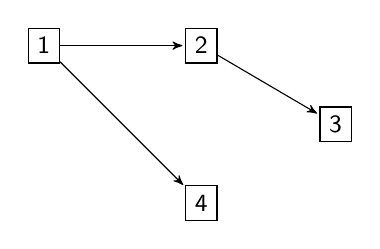
\begin{tikzpicture}[->,>=stealth',shorten >=1pt,auto,node distance=2cm,thin,
	bbl/.style={rectangle, draw, font=\sffamily\small}]
		\node[bbl] (1) {1};
		\node[bbl] (2) [right of=1] {2};
		\node[bbl] (4) [below of=2] {4};
		\node[bbl] (3) [right = 1.5cm of {$(2)!0.5!(4)$}] {3};
		
		\path[every node/.style={font=\sffamily\small}]
		(1) edge [right]node {} (2)
			edge [right]node {} (4)
		(2) edge [right]node {} (3);
	\end{tikzpicture}
	\caption{First Graph}
	\end{subfigure} %
	~
	\begin{subfigure}[b]{0.3\textwidth}
	\begin{tikzpicture}[->,>=stealth',shorten >=1pt,auto,node distance=2cm, thin,
	bbl/.style={rectangle, draw, font=\sffamily\small}]
		\node[bbl] (1) {1};
		\node[bbl] (2) [right of=1] {2};
		\node[bbl] (4) [below of=2] {4};
		\node[bbl] (3) [right = 1.5cm of {$(2)!0.5!(4)$}] {3};
		
		\path[every node/.style={font=\sffamily\small}]
		(1) edge [right]node {} (2)
		(2) edge [right]node {} (4)
		(4) edge [right]node {} (3);
	\end{tikzpicture}
	\caption{Second Graph}
	\end{subfigure}%
	~
	\begin{subfigure}[b]{0.3\textwidth}
	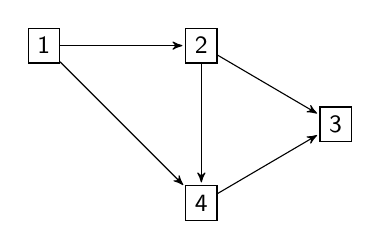
\begin{tikzpicture}[->,>=stealth',shorten >=1pt,auto,node distance=2cm, thin,
	bbl/.style={rectangle, draw, font=\sffamily\small}]	
		\node[bbl] (1) {1};
		\node[bbl] (2) [right of=1] {2};
		\node[bbl] (4) [below of=2] {4};
		\node[bbl] (3) [right = 1.5cm of {$(2)!0.5!(4)$}] {3};
		
		\path[every node/.style={font=\sffamily\small}]
		(1) edge [right]node {} (2)
			edge [right]node {} (4)
		(2) edge [right]node {} (3)
			edge [right]node {} (4)
		(4) edge [right]node {} (3);
	\end{tikzpicture}
	\caption{Merged Graph}
	\end{subfigure}
    \caption{Example Block Succession}
  \label{fig:bblsuc}

\end{figure}

%### 
\subsubsection{Memory Access Fitness Function}
%###
\label{sec:memcov}
All previously described fitness functions are aimed at increasing a coverage of one sort or another; however,
in the context of using \xmlmate to try and find vulnerabilities in the system under test, this is not
necessarily the most promising approach. In order to be able to find vulnerabilities having to do with
operations such as reading from and writing to memory, such as null pointer dereferences or buffer underflows
or overflows, the first na\"\i{}ve approach is to aim for a maximum number of memory reads and writes at a
maximum of addresses. This is the idea behind the \texttt{Memory Access} fitness function, which like its
cousin \texttt{Basic Block Coverage} fitness function, is a maximization function, with which it also shares
the \texttt{BinaryBackendFitnessFunction} as an ancestor. Once again, this fitness function consists of a
pintool and its complementary \java class. 

The pintool stores memory addresses that were accessed by the program under test in a set, which it sends to
the \java class upon test completion.
The \java class is very similar to that of its cousin fitness function, in fact they share the entirety of
their code.

However, upon consideration of the current use case, the distinction between test suites and tests as
prescribed by \evosuite no longer seems appropriate - what we actually want instead is to evolve a population
of single \xml files in order to find one individual file that triggers faulty behavior. To satisfy this newly
appeared need, the concept of a \emph{singleton population} was introduced.

Using a singleton population is a compromise between \evosuite's need for the presence of test suites to
evolve, and our need for only one set of files to be evolved. When the singleton population is used, the
population size of the genetic algorithm is limited to only one suite and the genetic algorithm itself is
modified accordingly, amongst other things by disabling elitism on the test suite level. Elitism is a
mechanism which ensures that the best individual (the best test suite in \evosuite's case) survives into the
next generation unaltered, so that fitness may never decrease from one generation to the next. Note,
that using elitism does not prevent the best individual from reproducing - its copies may do so freely, and
usually this is what leads to an improvement in fitness. 

With the singleton population in place, there is only one test suite to evolve, which means that the fitness
must now be calculated differently. The fitness of this single suite can no longer reflect the cumulative
result over all the tests, but must rather correspond to the fittest one of them, which, at the end of the
evolution, will be considered the result of the search, or the pinnacle of evolution, if you will.

This routine can be somewhat improved by adding a secondary evolution objective, which considers a
mutation of the test suite as an improvement even if it has the same number of memory accesses in the best
test, yet cumulatively its tests cause more unique memory addresses to be accessed. 

As a technical aside, I want to mention that there were considerations to model the use case of evolving a
set of files as a population of singleton test suites each containing a single file instead of the currently
employed population consisting of one suite. This, however, would have been unfavorable to the parallelization
efforts as per \cref{sec:par} because \evosuite does not allow parallel evaluation of test suites without some
major intrusion in its code base.
%### 
\subsubsection{Division by Zero Fitness Function}
%###
Like the \texttt{Memory Access} fitness function, the \texttt{Division by Zero} fitness function is also
designed to find vulnerabilities in the program under test instead of simply improving test input quality. In
particular, this fitness function aims to uncover a single class of denial of service vulnerabilities -
unhandled arithmetic exceptions that arise from performing division by zero.

When the program under test processes an input file, it usually executes multiple distinct division
instructions, and many of them - multiple times, so there is no simple and obvious way to directly assign a
fitness value to an input file. The first idea is to record all observed instances of division and choose the
smallest absolute value of a divisor as the fitness score. However, such an assignment is not very beneficial
to the diversity of the inputs' gene pool as it makes it converge to smaller files with a minimum number of
executed divisions as long as there is at least one divisor close to zero. Such a constriction opposes the
goal of triggering a division exception as it artificially and unnecessarily limits the number of sites
that are considered for exploration. 

To counteract this effect additional secondary objectives were put in place. The first secondary objective is
the \texttt{MaximizeDivisionsSecondaryObjective} and its goal is to enlarge the number of sites in the
program under test that are being explored by the search process by increasing the number of division
instructions covered by a suite. Using only this single secondary objective, however, leads to individuals
simply growing in size over the course of evolution, while keeping at least one close-to-zero divisor. While
this is beneficial to the diversity of the suites, it causes an unwelcome strain on the performance, which
is why another secondary - or rather a tertiary - objective has been added - the
\texttt{MinimizeCumulativeZeroDistanceSecondaryObjective}. The goal of this objective is to prevent an
uncontrolled growth and ensure overall improvement of quality of the individuals by keeping the cumulative
divisor distance to zero as small as possible.

At runtime the pintool component of the \texttt{Division by Zero} fitness function intercepts all invocations
of the \texttt{DIV} and \texttt{IDIV} x86 instructions and records the divisor value in a list, which is
associated with the address of the instruction in question by means of a map container. When the execution of
the system under test has ended, for each division instruction the pintool keeps only the divisor with the
smallest zero distance when it packages the message to be sent out to its \java fitness function counterpart.
There is a reason behind selecting the best divisor only after the main runtime instead of doing it on-the-fly,
even though it wastes some memory space for storing all observed divisors. This is an instance of the classical
runtime vs memory requirement trade off: by having injected code simply append any new value to a list
instead of doing comparisons to decide whether to keep or reject the new value, the code is simple enough to
be inlined and thus performs considerably faster; and with main memory being available in abundance on  modern
computers and execution speed being the most limiting factor, it seems like a good trade off to make.

Because the \texttt{Division by Zero} fitness function is meant to be used for vulnerability scanning, it is
exclusively compatible with the singleton population evolution mode introduced in \cref{sec:memcov}. The \java
component of this fitness function keeps a record of all executed division instructions alongside the absolute
value of their divisor closest to zero for each file in a suite. The overall fitness score of the entire suite
is then determined by finding the minimal divisor distance over all division instructions over all files in
the suite.

As previously suggested, this fitness function currently only supports integer based division instructions
because \pin imposes a limitation on retrieving floating point values from
registers\footnote{\url{https://software.intel.com/sites/landingpage/pintool/docs/67254/Pin/html/index.html\#FP}}.
Working around this and adding support for \texttt{SIMD} instructions are some planned future improvements.

An intuition is that it is unusual for valid well formed inputs to cause divisions by zero in the program under
test. It is therefore recommended to use the local search feature described in \cref{sec:local}, which is
capable of producing values beyond the range of validity, in order to increase the chances of actually
triggering arithmetic exceptions.

%### 
\subsubsection{Integer Overflow Fitness Function}
%### 
Continuing in the vein of fitness functions specialized in narrow categories of vulnerabilities, the next
fitness function is the \texttt{Integer Overflow Fitness Function}. Just as the name suggests, its aim is to
guide the evolution of inputs towards causing an unhandled integer overflow. Integer overflows are often
suitable as vessels for denial of service attacks as well as access control attacks, and therefore of
critical severity. 

In order to achieve its goal, the \texttt{Integer Overflow} fitness function uses its pintool component to
monitor all invocations of \texttt{MUL}, \texttt{IMUL} and \texttt{ADD} x86 instructions in the targeted
program and examine their arguments. Because overflows arise when two large integers are multiplied or added
such that the resulting value no longer fits in the size of an integer, this fitness function quite simply
favors larger arguments for those arithmetic operations. Quite similarly to the \texttt{Division by Zero}
fitness function, for each individual instruction a list of argument pairs is kept, from which the largest pair
is selected when reporting fitness to the \java master process. Once again, this is done for performance
reasons.
 
As this fitness function is also vulnerability-oriented, it is restricted to the singleton population usage
scenario; additionally, it is very advisable to employ the local search mechanism to encourage values
well outside the normal range of legal domains to increase the chance of triggering overflows.

This fitness function employs additional secondary objectives that are analogous to those of the
\texttt{Division by Zero} fitness function in that they also aim to increase the number of distinct
potential exploitation sites by favoring suites with a larger number of unique instructions, while limiting the
number of files in the suites to within a reasonable magnitude.

%### 
\subsubsection{Buffer Overflow Fitness Function}
%###
Yet another fitness function mainly aimed at its own specific class of vulnerabilities, the \texttt{Buffer
Overflow Fitness Function} seeks to identify potential buffer overflows and underflows, which can be highly
exploitable. This fitness function is very roughly based on the \texttt{Memory Access} fitness function,
however, it is somewhat more technically involved. 

The main idea behind aiming towards buffer overflows and underflows is deceptively simple: all one has to do
is monitor allocations, reallocations, and deallocations of buffers, record all memory accesses to them, and
favor those that are either at the beginning or end regions over those near the middle.

Unfortunately, the technical implementation of the prototypical pintool for use on Linux operating systems
turns out to be not as straightforward as the idea itself because, for the first time, an instrumentation on
function level is required. This is different from instrumenting applications on the level of individual
instructions or loading and unloading of binary images mainly because there exists a distinct possibility of
interleaved execution in multi-threaded applications. At least the technique for monitoring memory accesses
can be inherited from the \texttt{Memory Access} fitness function, so the focus of the problem at hand rests
with the potentially interleaved execution of \texttt{malloc}, \texttt{calloc} and \texttt{realloc} functions,
which are responsible for allocating buffers. 

Before considering concrete solutions, a data model for containing all relevant information must be designed.
For currently allocated buffers a set of \texttt{(rip, start, size)} triples will be kept, where \texttt{start}
and \texttt{size} are the beginning address and the size of the buffer, respectively, and \texttt{rip} is the
address of the instruction executed immediately after the return from the buffer allocating function, which is
used to provide both a distinction between different allocation sites, as well as a grouping criterion for
buffers that serve the same purpose at different times (think of buffer allocations in a loop for processing
subsequent chunks of an input). Logging of \texttt{rip}s arose from the need to uniquely identify different
allocation calls; unfortunately, \pin offers no easy possibility to identify the call site, but it provides
access to the \texttt{rip} out of the box. To ensure that only currently allocated buffers are stored, whenever
a buffer is freed by a call to \texttt{free}, the corresponding allocation is removed from the set of
recorded allocations.

This set is just an auxiliary data structure that does not provide any useful information in terms of the
planned fitness score. Therefore, another data structure is necessary for capturing the actual memory accesses
- an associative mapping from \texttt{rip}s to the maximum access distance from the center of a buffer
pertaining to an allocation before the \texttt{rip}. By using the distance from the center as a metric it
is possible to aim for accesses at both extremes of a buffer, thus giving equal preference to both overflows
and underflows at the same time. More specifically, the \texttt{access distance} of an access at address
\texttt{addr} to a buffer corresponding to the triple \texttt{(rip, start, size)} is calculated as $dist =
|start + \lfloor\frac{size}{2}\rfloor - addr|$. For an example consider \cref{fig:memaccess}: there is a buffer
corresponding to the triple \texttt{(any\_rip, 22, 27)} and two accesses \texttt{x} and \texttt{y} at
addresses 24 and 42 respectively. The center of this buffer is at address $22 + \lfloor\frac{27}{2}\rfloor =
35$. Thus, the access distance of \texttt{x} is $|35 - 24| = 11$ and that of \texttt{y} is $|35 - 42| = 7$.

\begin{figure}[H]
\centering
	\vspace{.5cm}
	\begin{bytefield}{32}
		\bitbox[]{6}{} & 
		\bitlabel{1}{\texttt{start}} &
		\bitbox[]{1}{} &  
		\bitlabel{1}{\texttt{x (dist = 11)}} &
		\bitbox[]{10}{} &  
		\bitlabel{1}{\texttt{center}} &
		\bitbox[]{6}{} &  
		\bitlabel{1}{\texttt{y (dist = 7)}} & 
		\bitbox[]{6}{} &  
		\bitlabel{1}{\texttt{start + size}} \\
		\bitheader[lsb=16]{22,24,35,42,49} \\
		\bitbox[tbr]{6}{\tiny ambient \\ \tiny variables} &
		\bitbox[tb]{2}{} &
		\bitbox[tb]{1}{\color{lightgray}\rule{\width}{\height}} &
		\bitbox[bt]{17}{\ \ \ \ \ \ \ \ \ \ \ \ \ \ \ \ \ \ buffer} &
		\bitbox[tb]{1}{\color{lightgray}\rule{\width}{\height}} &
		\bitbox[tbr]{6}{} &
		\bitbox[tbl]{6}{\tiny ambient \\ \tiny variables}
	\end{bytefield}
	\caption{Memory Access Distance}
	\label{fig:memaccess}
\end{figure}

Having established the desired data model and coming back to the problem of capturing buffer allocations as they
happen in a possibly multi-threaded application, a solution is to use {\small Pin's} API for instrumentation
at procedure level and have two callbacks - one at the entry of the allocation function, and the other at the
exit. With this setup the \texttt{rip} and the \texttt{size} values are accessible to the first callback and
\texttt{rip} and \texttt{start} to the second. So the idea is to reserve a triple \texttt{(rip, unknown, size)}
in the first callback, and later find it and fill in the \texttt{start} value in the second. Unfortunately, due
to interleaved execution, it is possible for two threads to enter an allocation function with the same
\texttt{rip} at the same time, so that when one of them returns activating the second callback, it has no way
of assigning the \texttt{start} value to the correct reserved entry. The obvious way to fix this is to
additionally keep the \texttt{thread\_id}, which, luckily, \pin also provides. This would somewhat bloat the
auxiliary data structure to a set of \texttt{(thread\_id, rip, start, size)} with probably very little
variation in the first value, so it seems like a waste of space. An optimization can be achieved by using
thread local storage facilities provided by \pin and reserve preliminary triples there, which requires
additional synchronization when moving the completed triples into the common auxiliary data structure. This
solution would be perfectly acceptable, if it weren't for a small comment in the examples section of {\small
Pin's}
documentation\footnote{\url{https://software.intel.com/sites/landingpage/pintool/docs/67254/Pin/html/\#Invocation}}:
\begin{quote}
{\small IPOINT\_AFTER} is implemented by instrumenting each return instruction in a routine. \pin tries to find
all return instructions, but success is not guaranteed.
\end{quote}
Unfortunately, {\small IPOINT\_AFTER} is exactly the instrumentation point needed to implement the second
callback, which makes the entire contraption unreliable at best and simply wrong at worst.

Luckily, a better solution presented itself - it is possible to replace the allocating functions with variants
that additionally perform the record keeping task.
This is actually exactly what is already used for communicating between the test drivers and their pintools, as
mentioned in \cref{sec:components}, when the pintool replaces the well known functions in the test driver with
its own versions. Except in this case an additional feature of procedure replacement was used: the signature
change. This is best explained on a simple example of the \texttt{malloc} function. 

The original version has the signature \mintinline{cpp}{void *malloc(size_t size)}. In order to be able to
record the \texttt{rip} of an invocation, the malloc wrapper function has to have a signature of 
\mintinline{cpp}{void *mallocWrapper(size_t size, void *rip)}, whereby \pin would fill in the second argument
at the moment of invocation. The code of this wrapper function is roughly sketched in \cref{lst:mallocwrapper}.

\begin{listing}[h]
\centering
\begin{cppcode}
void *MallocWrapper(size_t size, void *rip) {
	void *start = malloc(size); // call original malloc
	allocations.insert(Allocation_T(rip, start, size)); // store triple
	return start; // return original value
}
\end{cppcode}
\caption{MallocWrapper Code Sketch}
\label{lst:mallocwrapper}
\end{listing}

The wrapper function first invokes the original \texttt{malloc} and stores its return value. At this point the
wrapper has access to all three necessary values at once and stores the triple \texttt{(rip, start, size)}
before returning the original return value. Please regard the presented code as pseudocode because the actual
code is somewhat more involved.

Firstly, calling the original \texttt{malloc} function is not as straightforward because \pin has its own
implementation of malloc that uses its own allocator and thus is not compatible with the intended
\texttt{malloc} call as any attempt to free the returned buffer from inside the instrumented program using a
call to its \texttt{free} function will result in a segmentation error. Additionally, the space reserved for
\pin allocations is rather limited, which also makes it infeasible to patch the \texttt{free} calls
accordingly. Even if \pin did not override \texttt{malloc}, simply inserting a call to it would result in an
infinite loop as \pin would try to replace this call by the wrapper as well. Therefore the invocation is
actually a call to a special method in {\small Pin's} API that allows execution of the original function
without it being instrumented.

Secondly, additional checks are performed inside the wrapper, such as ensuring that only calls pertaining to
the targeted binary image are recorded or testing the return value for being \texttt{NULL} and treating this
case specially.

The allocation functions \texttt{calloc} and \texttt{realloc} are treated analogously to \texttt{malloc}, but
\texttt{free} is actually not replaced at all because it is sufficient to add a callback at its entry site
(which, luckily, \pin guarantees to work) that will simply remove a triple with the \texttt{start} value equal
to the argument of \texttt{free} if one is found.

As mentioned previously, the fitness information the pintool of the \texttt{Buffer Overflow
Fitness Function} sends to its \java counterpart is the memory access map, which, in contrast to the
\texttt{Division by Zero} and \texttt{Integer Overflow} fitness functions is updated in-place and not only
after the processing of an input file. Because memory accesses are much more numerous than e.g. \texttt{DIV}
or \texttt{MUL} instruction invocations, the reasonable choice in the memory-speed trade off is somewhat offset.

The \java part of this fitness function tries to maximize the maximum distance of the accesses from their
respective buffer's centers, and by employing additional secondary objectives, it also aims to enlarge the
number of accessed buffers as well as the cumulative access distance in a suite, while preventing the suites
from bloating by favoring smaller ones if all their previously mentioned characteristics are equal.

As is the case with several previous fitness functions, this fitness function is also geared towards finding
vulnerabilities and employs the singleton population paradigm and benefits greatly from enabling local search -
in this case especially so. It would be infeasible to count memory accesses outside allocated buffer ranges as
out-of-bounds accesses to the buffers themselves because they may well be just accesses to ambient variables.
Therefore this fitness function assigns maximum values to accesses just at the legal bounds of the buffers and
the small mutations caused by the local search mechanism make it possible to break out of this restriction
by a small amount and thus possibly trigger a sought-after vulnerability.

\section{Evaluation}
\label{sec:evaluation}
\subsection{Subjects}
\tocless\subsubsection{libxml2}
\tocless\subsubsection{libpng}
\tocless\subsubsection{libpcap}
%\subsubsection{libflac}
\subsection{Results}
\subsection{Threats to Validity}
\section{Conclusion}
\label{sec:conclusion}
% \section{Future Work}
% \label{sec:future}
The presented work paves the way for many more useful improvements and extensions on numerous facets and
aspects of \xmlmate. The following gives a brief overview of some of the most interesting future work items.

%###
\paragraph{Complete Parallelization} ~\\
%###
One particularly large work item is rewriting the
genetic algorithm of \xmlmate from scratch aiming for more comprehensive parallelization support from the
beginning.
At the time of writing it is estimated that this goal is best achieved by making heavy use of many of the features that the
Scala\cite{scala-overview-tech-report} programming language has to offer, as well as utilizing the Akka actor-based message-driven concurrency framework\cite{Wyatt:2013:AC:2663429} to make \xmlmate fully
concurrent and distributed.
%###
\paragraph{Meta-Heuristics} ~\\
%###
To make better use of the available computational resources, the genetic algorithm at the heart of
\xmlmate can profit from the addition of meta-heuristics that would govern the number of instances of certain
subprocesses like format converters or worker nodes during runtime based on the proportion of their
respective load on the system.
%###
\paragraph{Specification Violation} ~\\
%###
Delving deeper into the use case of finding vulnerabilities, it might be wise to further investigate
the mechanism responsible for generating aberrant and unexpected input values and extend it to work not only
with integer and floating point types, but other types and even structures permissible in \xml as well.
%###
\paragraph{Further Fitness Functions} ~\\
%###
Since \xmlmate provides an interface for pluggable fitness functions, it is only natural to want to try
out more of them. Some next candidates would be the branch coverage fitness function as implemented in
\evosuite in the context of generating test suites, and for program resilience testing purposes a fitness
function that aims to maximize the number of context switches in a concurrent program seems interesting for
finding multi-threading related issues such as deadlocks, livelocks, starvation and the like.
%###
\paragraph{Hardware Counters and Virtualization} ~\\
%###
For future fitness functions that use program performance values in the computation of their
fitness score it is possible to significantly increase efficiency by making use of hardware performance
counters. These are usually provided by modern hardware and can be directly accessed in most operating systems
by means of special APIs like the ones provided by the PAPI\cite{Mucci99papi:a} or LTTng\cite{
combined_tracing_ols2009} libraries. Note that this would impose a limitation on the concurrent use of \xmlmate
on a single machine; however, this limitation can probably be solved by using virtualization techniques such as
Docker\cite{docker} -- especially since \xmlmate is now a
distributed system capable of running across multiple distinct hardware nodes. This arrangement can also be of
special benefit to creating a fitness function specialized in detecting buffer overflows by means of advanced
operating system features like memory page marking and eviction. One library specializing in such techniques
of memory debugging is DUMA\footnote{\url{http://sourceforge.net/projects/duma/}}, which can be seen as a
successor of the discontinued Electric Fence project.
%###
\paragraph{More Efficient Message Transport} ~\\
%###
If \xmlmate is going to be used in truly distributed systems, it is probably a good idea to replace
the currently employed \msgpack message serialization and deserialization engine by another, more efficient and
sophisticated library. When real network traffic is involved, it seems like a good idea to minimize the amount
of traffic that has to pass through the network, and having a library with a streaming interface that
additionally allows to partially deserialize messages before they have reached their destination completely is
certainly also of good use as well. Some candidate replacements can be found in \cref{sec:msgpack}.
%###
\paragraph{Robust Communication} ~\\
%###
Further elaborating upon the idea of distributed execution environments in the presence of unreliable
nodes, it seems wise to invest some effort into extending the inter-component communication protocol for
reliability and message delivery guarantees.
%###
\paragraph{Additional Test Subjects} ~\\
%###
With more fitness functions come more test subjects that can be explored. For formats, for which the
corresponding schemas and converters already exist in the current version, such applications as \emph{tcpdump}
and \emph{tshark} for the \pcap format and a whole
lot\footnote{\url{http://www.libpng.org/pub/png/pngapcv.html}} of programs for \png are available.
Adding test subjects that process other file formats requires adding new schemas and converters that
support them. Some envisioned targets are \emph{libjpeg}, \emph{giflib} and \emph{libflac} libraries for
processing image, animation and sound files, respectively.
%###
\paragraph{Result Minimization} ~\\
%###
In terms of usability and convenience \xmlmate could profit from minimizing the files responsible for
revealing a defect in the application under test using delta debugging\cite{zeller2002simplifying} to make it
easier for the user to find the actual cause of the failure in question.
%###
\paragraph{Crossing the Programming Language Barrier} ~\\
%###
Ending on another big topic, seeing as \xmlmate has its origins in the \java world, it could be extended
to support testing of \java applications that use native code by performing instrumentation on both \java
byte code and the native binary code. 

{\color{white}{Thank you for reading the digital version and not printing this out on paper! :)}}
\newpage
\section*{References}
\renewcommand\refname{}
\addcontentsline{toc}{section}{References}
\bibliographystyle{plain}
\bibliography{sources}
\newpage
\listoftodos[Notes] % TODO remove ;)
\end{document}
